\section{Exercise 1 - Closed Form Expressions}
\subsection{$\sum_{i=0}^d k^i \quad \mathrm{for } \, k>0$ (Ex1.1)}
\begin{equation}
\begin{aligned}
    \sum_{i=0}^d k^i &= \sum_{i=0}^d k^i \\
    \sum_{i=0}^d k^i - k \sum_{i=0}^d k^i &= \sum_{i=0}^d k^i - k \sum_{i=0}^d k^i \\
    \sum_{i=0}^d k^i - k \sum_{i=0}^d k^i &= \sum_{i=0}^d k^i - \sum_{i=1}^{d+1} k^i \\
    \sum_{i=0}^d k^i \, (1-k) &= 1 - k^{d+1}\\
    \sum_{i=0}^d k^i   &=  \frac{k^{d+1} - 1}{k-1}
    \label{closedForm_Ex1.1}
\end{aligned}
\end{equation}

\subsection{$\sum_{i=1}^d ik^i \quad \mathrm{for } \, k>0$ (Ex1.4)}
\begin{equation}
\begin{aligned}
    \sum_{i=1}^d ik^i &= \sum_{i=0}^d ik^i = 
    \sum_{i=0}^d k \frac{\mathrm{d}}{\mathrm{d}k}k^i =
    k \frac{\mathrm{d}}{\mathrm{d}k} \overbrace{\sum_{i=0}^d k^i}^{\text{use (\ref{closedForm_Ex1.1})}} \\
    \sum_{i=1}^d ik^i &= k \frac{\mathrm{d}}{\mathrm{d}k} \frac{1 - k^{d+1}}{1-k} = 
    \frac{d  k^{d+2} - (d+1)k^{d+1} + k}{(1-k)^2}
    \label{closedForm_Ex1.4}
\end{aligned}
\end{equation}

\subsection{$\sum_{i=1}^d i2^{d-i}$ (Ex1.3)}
\begin{equation}
    \begin{aligned}
        \sum_{i=1}^d i2^{d-i} &, \quad \text{use k instead of 2} \\
        \sum_{i=1}^d ik^{d-i} &= \sum_{i=0}^d dk^{d-i} - \sum_{i=0}^d (d-i)k^{d-i} \\
        &= d\underbrace{\sum_{j=0}^d k^{j}}_{\text{use } (\ref{closedForm_Ex1.1})} - 
        \underbrace{\sum_{j=0}^d jk^{j}}_{\text{use } (\ref{closedForm_Ex1.4})} \quad \text{with } j := d-1 \\
        &= \frac{d(k^{d+1} - 1)}{k-1} - \frac{d  k^{d+2} - (d+1)k^{d+1} + k}{(1-k)^2} \quad \text{set $k$ back to 2} \\
        &= d2^{d+1} - d - d2^{d+2} + d2^{d+1} + 2^{d+1} - 2 \\
        \sum_{i=1}^d i2^{d-i} &= 2^{d+1} -2 - d
        \label{closedForm_Ex1.3}
    \end{aligned}
    \end{equation}

\subsection{$\sum_{i=1}^d i2^i$ (Ex1.2)}

\begin{equation}
    \begin{aligned}
        \sum_{i=1}^d i2^i = d  2^{d+2} - (d+1)2^{d+1} + 2 \quad \text{with use of (\ref{closedForm_Ex1.4})}
    \end{aligned}
\end{equation}

\pagebreak

\section{Exercise 2 - Graph Tree's with Canonical Numbering}
\subsection{$T^d_k$ with $k=3$ and $d=3$}

\begin{figure}[h]
    \begin{center}
        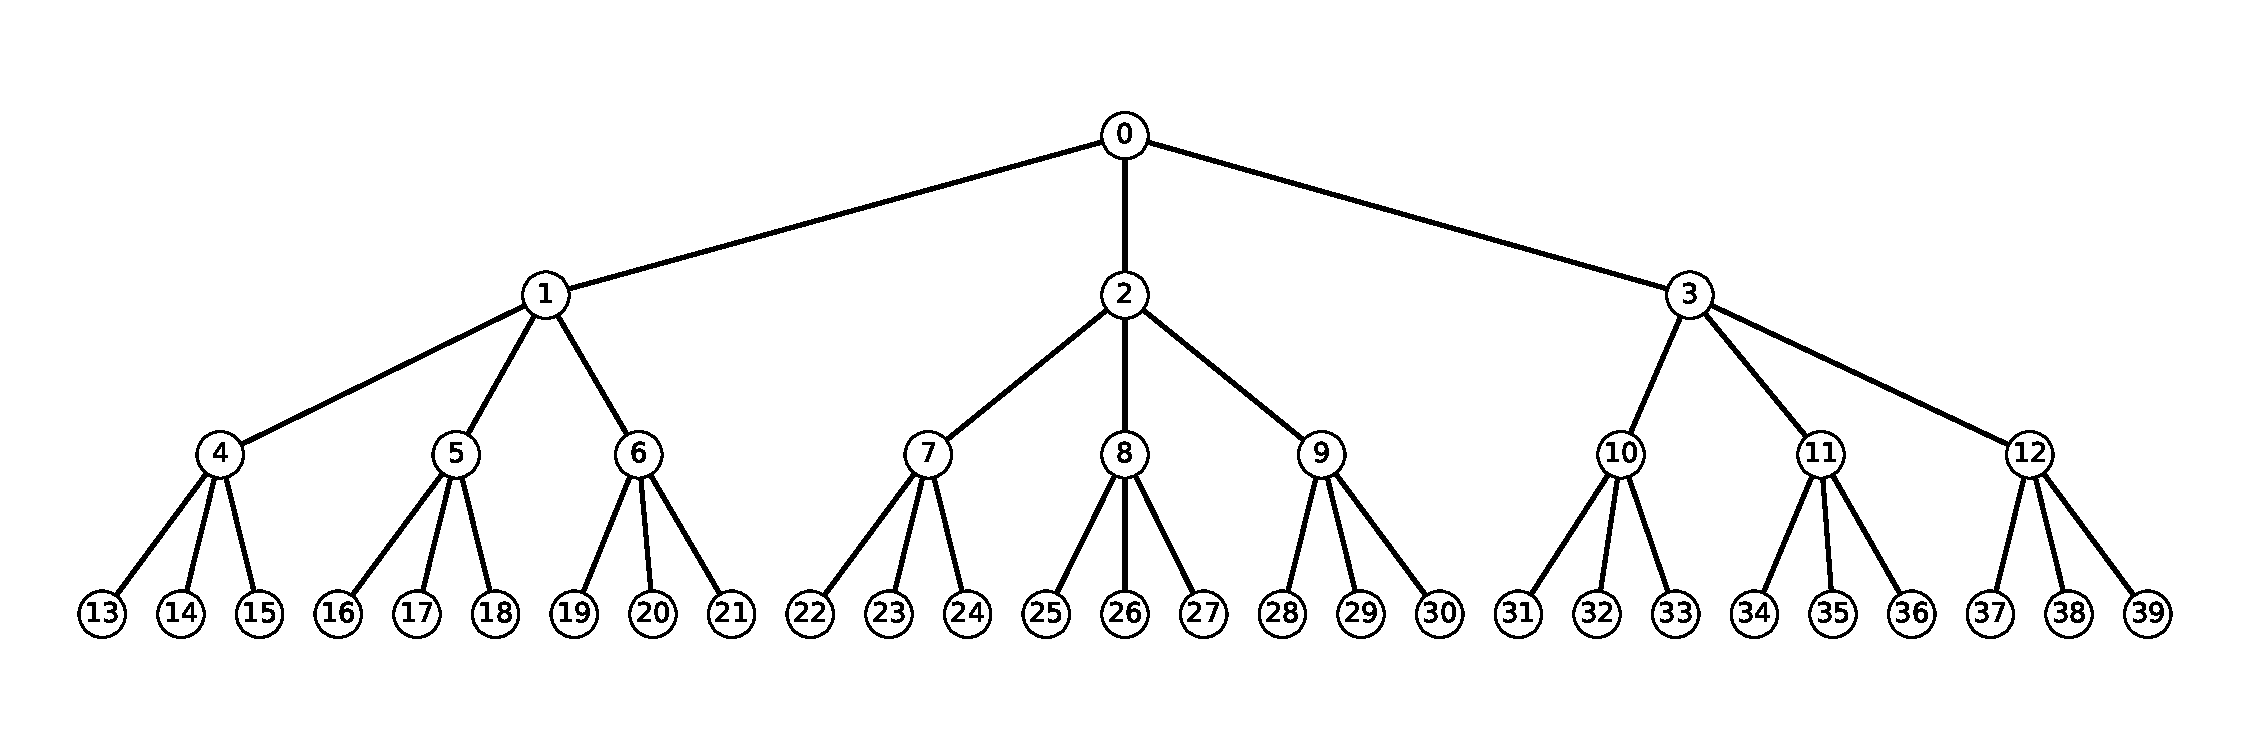
\includegraphics[width=\linewidth]{figures/Ex1_2_a.pdf}
        \caption{Fixed-degree k-ary heigh $d$ tree $T^d_k$ with $k=3$ and $d=3$}
    \end{center}
\end{figure}


\subsection{$B^d_k$ with $k=3$ and $d=4$}

\begin{figure}[h]
    \begin{center}
        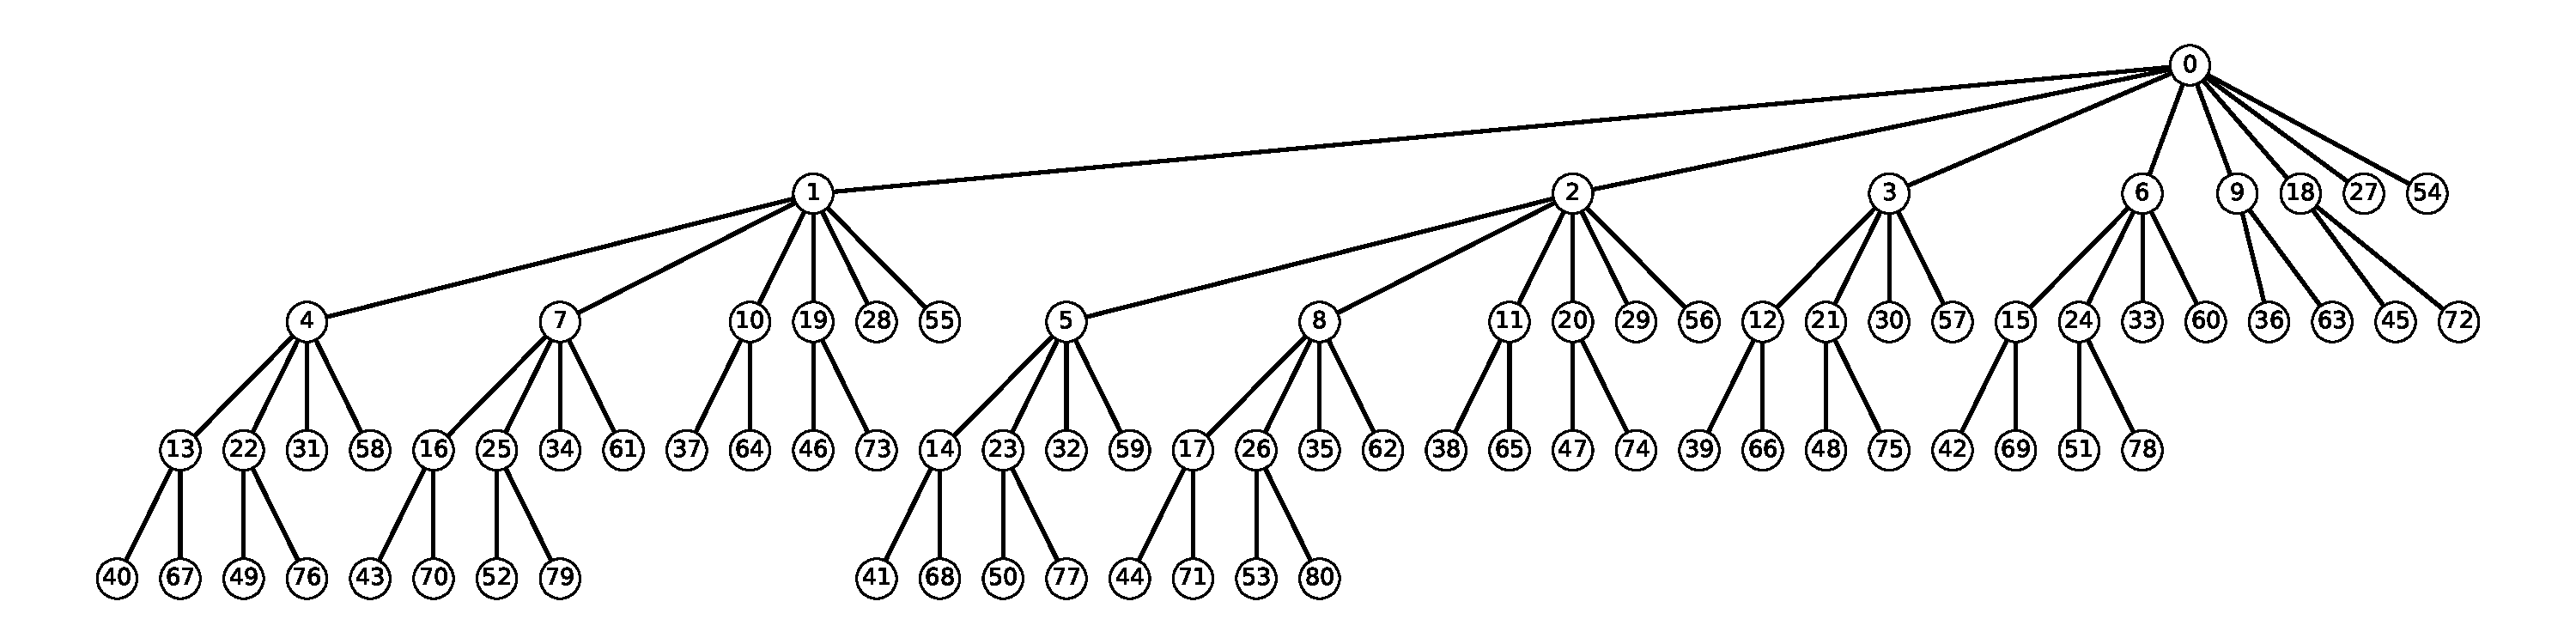
\includegraphics[width=\linewidth]{figures/Ex1_2_b.pdf}
        \caption{Complete heigh $d$ k-nomial tree $B^d_k$ with $k=3$ and $d=4$}
    \end{center}
\end{figure}

\subsection{Complete unbalanced binary tree}
The tree drawn below is following the Pre-Order numbering scheme.

\begin{figure}[h]
    \begin{center}
        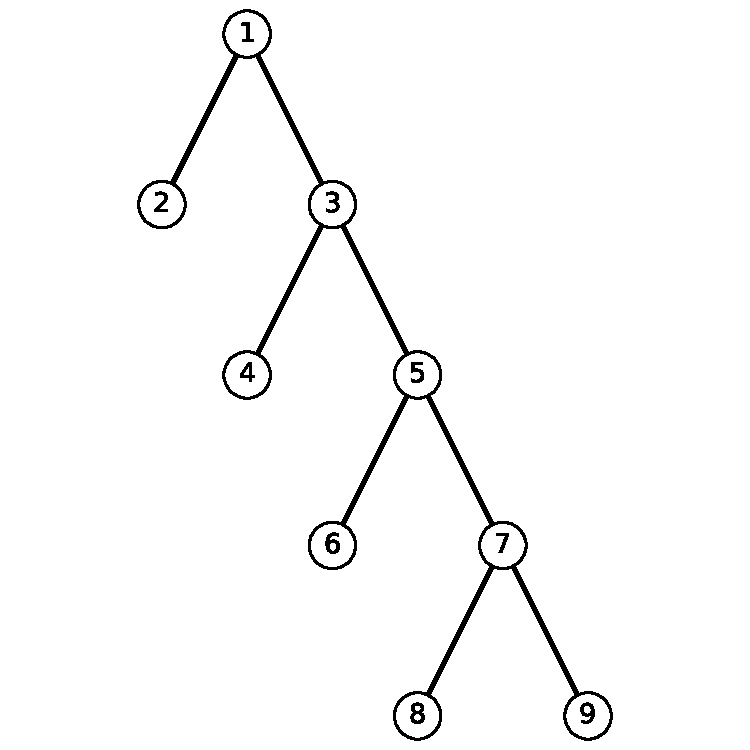
\includegraphics[width=0.3\linewidth]{figures/Ex1_2_c.pdf}
        \caption{Complete (but unbalanced) binary tree of height $d = 4$ with $p = 9$ nodes.}
    \end{center}
\end{figure}

\pagebreak

\section{Exercise 3 - Planar Graph $H_d$}
For which $d$ is the hypercube $H_d$ a planar graph? In graph theory, a planar graph is a graph that can be embedded in the plane, i.e., 
it can be drawn on the plane in such a way that its edges intersect only at their endpoints. In other words, it can be drawn in such a way 
that no edges cross each other. in fact this works for $d \le 3$. It can also be shown with Wagner's theorem.

\begin{figure}[h]
    \begin{center}
        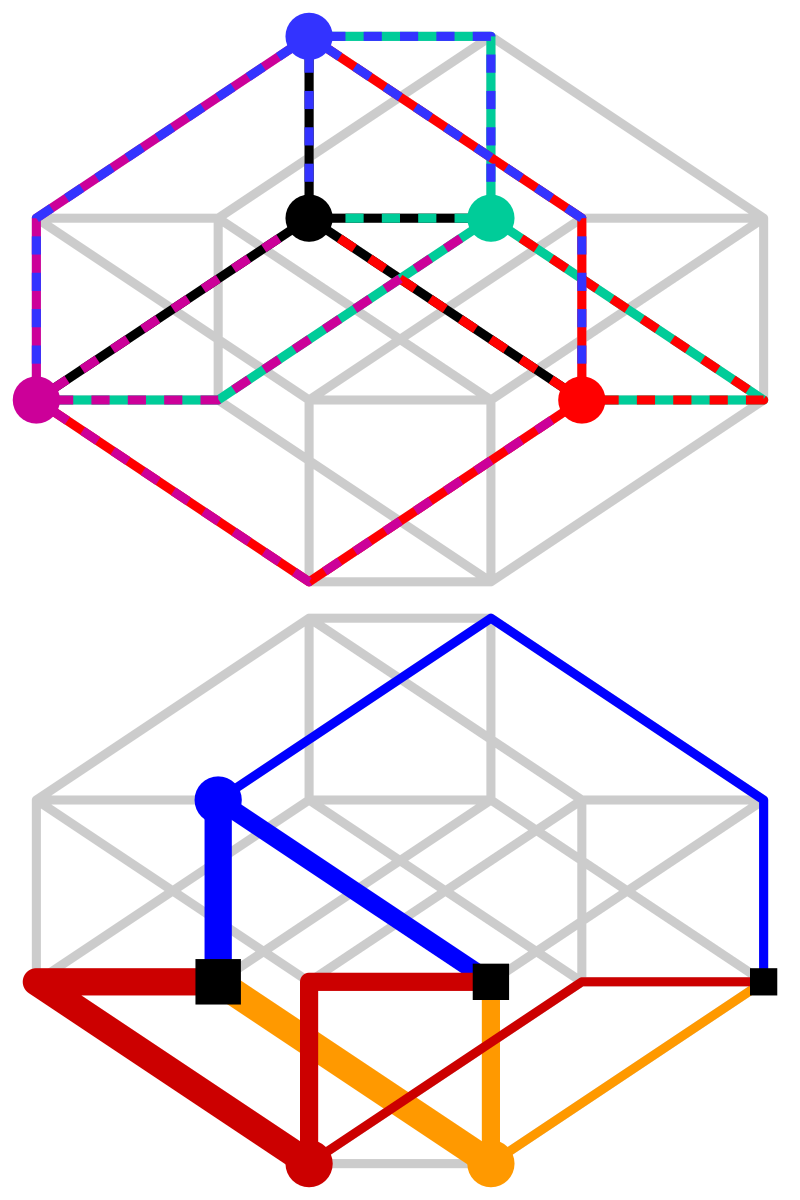
\includegraphics[width=0.3\linewidth]{figures/Ex1_3.png}
        \caption{Proof without words that a hypercube graph is non-planar Wagner's theorems and finding either $K_5$ (top) or $K_{3,3}$ (bottom) subgraphs \cite{Wagners_theorem}}
    \end{center}
\end{figure}

In fact for all hypercubes up to $d \le 3$, neither $K_5$ nor $K_{3,3}$ can be found embedded in the hypercube. \linebreak \qed

\pagebreak

\section{Exercise 4 - Gray Code Embedding in a Hypercube}
The Gray code algorithms 2 and 3 from the HPC script are implemented in C and shown in the listing below. The executed binary indeed yields
the console output \texttt{yarg and gray did not throw errors - Ex1.4 done :-)}.

\begin{lstlisting}[language=C, title=C Language Listing for EX1.4 ]
#include <stdio.h>
#include <math.h>
typedef unsigned int uint;
uint gray(uint num)
{
    return num ^ (num >> 1); 
}
uint yarg(uint num)s
{
    uint mask = num;
    while (mask)
    { 
        mask >>= 1;
        num ^= mask;
    }
    return num;
}
uint yarg32(uint num)
{
    num ^= num >> 16;
    num ^= num >> 8;
    num ^= num >> 4;
    num ^= num >> 2;
    num ^= num >> 1;
    return num;
}
int main()
{
    int d = 20;
    uint old = gray(0);
    for (int j = 1; j < pow(2, d); j++)
    {
        uint ans = gray(j);
        uint diff = old ^ ans;
        int check = 0;

        for (int k = 0; k < d; k++)
        {
            if (diff == (1 << k))
            {
                check++;
            }
        }
        if (check != 1)
        {
            printf("gray() error");
            break;
        }
        if (yarg(ans) != j)
        {
            printf("yarg() error");
            break;
        }
        old = ans;
    }
    printf("yarg and gray did not throw errors - Ex1.4 done :-)!\n");
    return 0;
}
\end{lstlisting}